% Search for all the places that say "PUT SOMETHING HERE".

\documentclass[11pt]{article}
\usepackage{amsmath,textcomp,amssymb,graphicx,enumerate,hyperref,enumitem,mathtools,tikz-qtree,listings,tikz}

\def\Name{Jonathan Sun}  % Your name
\def\SID{25020651}  % Your student ID number
\def\Homework{3} % Number of Homework
\def\Session{Fall 2017}


\title{CS170 --- \Session --- Homework \Homework \space Solutions}
\author{\Name, SID \SID}
\markboth{CS170 --- \Session --- Homework \Homework \space --- \Name}{CS170 --- \Session --- Homework \Homework --- \Name}
\pagestyle{myheadings}
\date{}

\def\endproofmark{$\Box$}
\newenvironment{proof}{\par{\bf Proof:}}{\endproofmark\smallskip}
\newenvironment{FourPartSolution}{\par{\bf Four-Part Solution:}}{\smallskip}
\newenvironment{mainIdea}{{\bf Main Idea:}}{\smallskip}
\newenvironment{pseudocode}{\par{\bf Pseudocode:}}{\smallskip}
\newenvironment{proofOfCorrectness}{\par{\bf Proof of Correctness:}}{\endproofmark\smallskip}
\newenvironment{runTime}{{\bf Run Time:}}{\smallskip}
\newenvironment{justification}{\par{\bf Justification:}}{\smallskip}
% \newenvironment{proofOfCorrectness}{\par{\bf Proof of Correctness:}}{\endproofmark\smallskip}
% \newenvironment{runTime}{\par{\bf Run Time:}}{\smallskip}
% \newenvironment{justification}{\par{\bf Justification:}}{\smallskip}

\usepackage[margin=1in]{geometry}



\begin{document}
\maketitle

\section*{0. Who Did You Work With?}

Collaborators: Kevin Vo, Aleem Zaki, Jeremy Ou



\newpage
\section*{1. Can you win OneSeventy?}
\vspace*{1\baselineskip}
\begin{mainIdea}
\vspace*{1\baselineskip}
\\
My main idea for this problem is to run DFS twice, once on the graph and once on a `source' node. When I run DFS the first time, I run it on the graph of $N$ quests enumerated as ${n_1, n_2, ..., n_N}$. Doing so will find me the `source' node, or a node with no incoming edges, since the `source' node is the node with the last postvisit number.
\\
When I run DFS the second time, I will run it on the `source' node rather than on all the quests. If I find that the last postvisit number is on that same `source' node then I know that I have traversed through the entire graph and returned back to the `source' node I started from. This means that the game is winnable. If the last postvisit number is not found on the same `source' node then I know that I have not traveresed through all nodes, or quests, and therefore the game is not winnable.
\end{mainIdea}
\vspace*{1\baselineskip}
\\
\begin{runTime}
\vspace*{1\baselineskip}
\\
$O(|V| + |E| + |V| + |E|) = O(2|V| + 2|E|) = O(|V| + |E|)$.
\vspace*{1\baselineskip}
\\
The runtime is $O(|V| + |E|)$ because we are running DFS twice. Running DFS once has a run time of $O(|V| + |E|)$ and since we are running DFS twice we get a run time of $O(|V| + |E| + |V| + |E|) = O(2|V| + 2|E|) = O(|V| + |E|)$.
\end{runTime}


\newpage
\section*{2. Graph Basics}
\begin{enumerate}[label=(\alph*)]
\item
Yes. The algorithm to find the shortest path between $s$ and $t$ may have terminated before hitting $t'$ or $t'$ was never going to be hit in the first place when going from $s$ to $t'$.

\item
No. The algorithm will not be guaranteed to return the same solution because the more edges there are in the solution for the shortest path, it increases more compared to just adding $k$ to the original total length of the shortest path. The following example shows why:
\vspace*{1\baselineskip}
\\
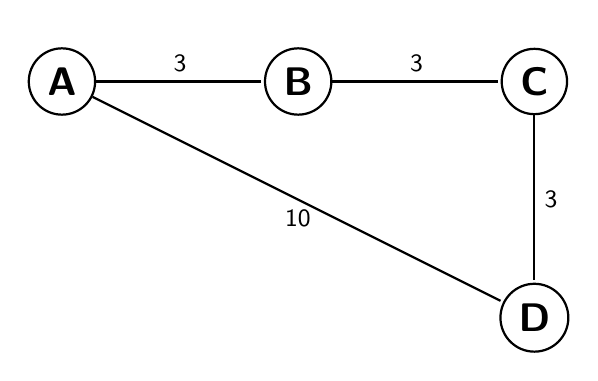
\begin{tikzpicture}[shorten >=1pt, auto, node distance=3cm, thick, main node/.style={circle, draw, font=\sffamily\Large\bfseries}]
	\node[main node, label] (A) {A};
	\node[main node, label] (B) [right of=A] {B};
	\node[main node, label] (C) [right of=B] {C};
	\node[main node, label] (D) [below of=C] {D};

	\path[every node/.style={font=\sffamily\small}]
		(A) edge node [above] {3} (B)
			edge node [below] {10} (D)
		(B) edge node [above] {3} (C)
		(C) edge node [right] {3} (D);
\end{tikzpicture}
\\
Running Dijkstra's algorithm from $A$ to $D$ will return $A$, $B$, $C$, $D$. However, adding $5$ to the lengths of all edges gives us:
\\
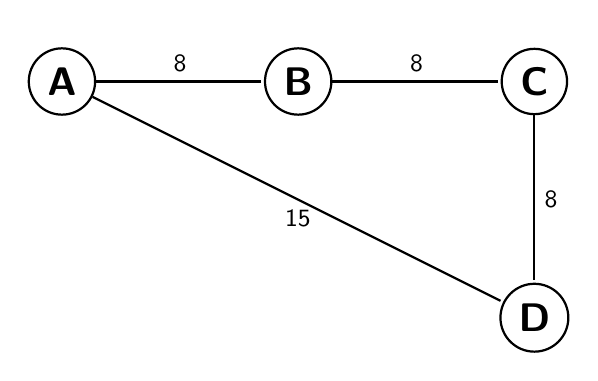
\begin{tikzpicture}[shorten >=1pt, auto, node distance=3cm, thick, main node/.style={circle, draw, font=\sffamily\Large\bfseries}]
	\node[main node, label] (A) {A};
	\node[main node, label] (B) [right of=A] {B};
	\node[main node, label] (C) [right of=B] {C};
	\node[main node, label] (D) [below of=C] {D};

	\path[every node/.style={font=\sffamily\small}]
		(A) edge node [above] {8} (B)
			edge node [below] {15} (D)
		(B) edge node [above] {8} (C)
		(C) edge node [right] {8} (D);
\end{tikzpicture}
\\
Running Dijkstra's algorithm from $A$ to $D$ will return $A$, $D$ instead of $A$, $B$, $C$, $D$.

\item
No. If an edge length becomes negative, then Dijkstra’s algorithm will not work. An example is shown below:
\\
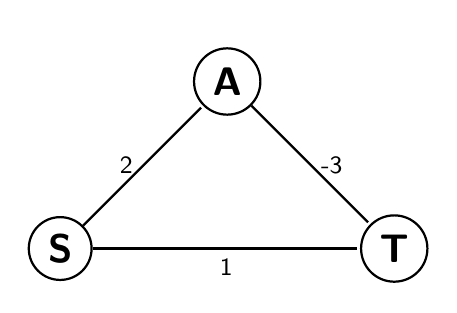
\begin{tikzpicture}[shorten >=1pt, auto, node distance=3cm, thick, main node/.style={circle, draw, font=\sffamily\Large\bfseries}]
	\node[main node, label] (A) {A};
	\node[main node, label] (S) [below left of=A] {S};
	\node[main node, label] (T) [below right of=A] {T};
	\path[every node/.style={font=\sffamily\small}]
		(A) edge node [right] {-3} (T)
		(S) edge node [left] {2} (A)
			edge node [below] {1} (T);
\end{tikzpicture}
\\
Running Dijkstra's algorithm from starting node $S$ and end node $T$ gives us $S$, $T$ instead of the correct solution of $S$, $A$, $T$.

\item
Yes. The algorithm will still work if you multiply all the edges by the same positive number $k$. The reason is that if the path is the sum of all the edges in the shortest path solution given by Dijkstra's algorithm, then multiplying all edges in the path by a scalar is equivalent to multiplying the total edge length in the path by that scalar due to the distributive property. In other words, multiplying all the edges by the same positive number $k$ is equivalent to just stretching the graph out.
\end{enumerate}



\newpage
\section*{3. Graph Basics}
\begin{enumerate}[label=(\alph*)]
\item
To show that an undirected graph is bipartite if and only if it has no odd cycles, I will consider a base case. The base case will be a simple graph where a start node, $n_1$, from subset $A$ is connected to $n_2$ in subset $B$. This node in subset $B$ is connected to $n_3$ in subset $A$ that is not the start node. The base case is shown in the graph below:
\\
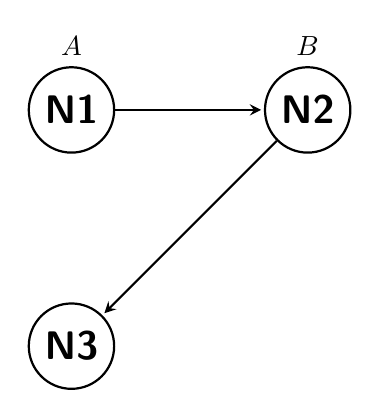
\begin{tikzpicture}[->, >=stealth, shorten >=1pt, auto, node distance=3cm, thick, main node/.style={circle, draw, font=\sffamily\Large\bfseries}]
	\node[main node, label=above:$A$] (N1) {N1};
	\node[main node, label=above:$B$] (N2) [right of=N1] {N2};
	\node[main node, label] (N3) [below of=N1] {N3};
	\path[every node/.style={font=\sffamily\small}]
		(N1) edge node [] {} (N2)
		(N2) edge node [] {} (N3);
\end{tikzpicture}
\\
In this base case, it is clear that there are $2$ edges in total, which is an even number.
\vspace*{1\baselineskip}
\\
At this point, I can either continue the graph or complete the graph. I will first continue the graph. To continue the graph, I will attempt to add another node in subset $A$. Before I can do that, however, I need to add another node, $n_4$, in subset $B$ since every edge in $G$ must cross between $A$ and $B$ and therefore the nodes must alternate between being in subset $A$ or being in subset $B$. Following $n_4$ will be $n_5$, the node I wanted to add into subset $A$. Because I will add $2$ more nodes into the graph, this means that I will also add $2$ more edges into the graph. This case is shown in the graph below:
\\
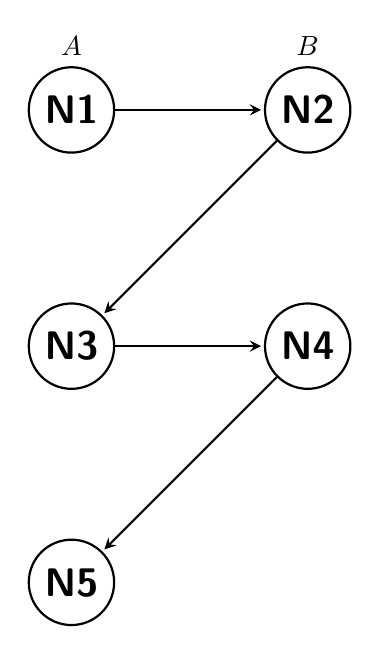
\begin{tikzpicture}[->, >=stealth, shorten >=1pt, auto, node distance=3cm, thick, main node/.style={circle, draw, font=\sffamily\Large\bfseries}]
	\node[main node, label=above:$A$] (N1) {N1};
	\node[main node, label=above:$B$] (N2) [right of=N1] {N2};
	\node[main node, label] (N3) [below of=N1] {N3};
	\node[main node, label] (N4) [below of=N2] {N4};
	\node[main node, label] (N5) [below of=N3] {N5};
	\path[every node/.style={font=\sffamily\small}]
		(N1) edge node [] {} (N2)
		(N2) edge node [] {} (N3)
		(N3) edge node [] {} (N4)
		(N4) edge node [] {} (N5);
\end{tikzpicture}
\\
It is clear that on top of the original $2$ edges in the base case, I have added another $2$ edges in total, which is an even number. Therefore, to continue the graph I will end up adding an even number of edges to an even number of edges which is still an even number of total edges.
\\
Next, I will show what happens when you choose to complete the graph on the base case. To complete the graph, I will need to end with an edge going into the starting node $n_1$, which is in subset $A$. Doing so means that the second to last node must be added into subset $B$ since the second to last node must not be in subset $A$. Therefore, I will need to add $n_4$ into subset $B$, which adds $2$ more edges into the graph. This case is shown in the graph below:
\\
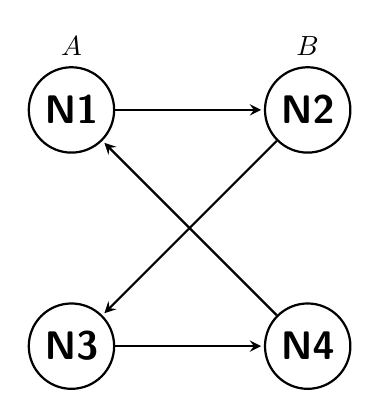
\begin{tikzpicture}[->, >=stealth, shorten >=1pt, auto, node distance=3cm, thick, main node/.style={circle, draw, font=\sffamily\Large\bfseries}]
	\node[main node, label=above:$A$] (N1) {N1};
	\node[main node, label=above:$B$] (N2) [right of=N1] {N2};
	\node[main node, label] (N3) [below of=N1] {N3};
	\node[main node, label] (N4) [below of=N2] {N4};
	\path[every node/.style={font=\sffamily\small}]
		(N1) edge node [] {} (N2)
		(N2) edge node [] {} (N3)
		(N3) edge node [] {} (N4)
		(N4) edge node [] {} (N1);
\end{tikzpicture}
\\
It is clear that on top of the original $2$ edges in the base case, I have added another $2$ edges in total, which is an even number. Therefore, to continue the graph I will end up adding an even number of edges to an even number of edges which is still an even number of total edges.
\vspace*{1\baselineskip}
\\
Therefore, this shows that a graph is bipartite if and only if it has no odd cycles since there can only be even cycles. Continuing a cycle or ending a cycle ends up adding an even number of edges to a graph with an even number of edges since the nodes must alternate between being in subset $A$ and in subset $B$.



\item
Since the graph is a DAG, then there is a possible topological ordering for this graph and therefore a source node exists. This also means that the source node is first in the topological sort and that every other node will follow it. There should exist an edge from the source to every other vertices in the graph, from the statement of it being a semiconnected graph. Therefore, if we `pop' the source node and have the next item in the topological sort be the new source node, then this new source node will also have an edge to every other vertices. Therefore, we can say that for every node in the topological sort, there exists an edge between this source node and every node that comes after it in the source. This means that a semiconnected graph implies a direct path that visits all vertices in the graph. However, I need to also show that if there exists a directed path that visits all the vertices in the graph, then this implies that the graph is a semiconnected graph.
\vspace*{1\baselineskip}
\\
To show that if there exists a directed path that visits all the vertices in the graph, then this implies that the graph is a semiconnected graph, I need to show that the graph only has a single source. If it has two sources, then the graph is not a semiconnected graph because the two source nodes cannot visit each other. Therefore, if you have a source node and there is a path that visits every other vertex, then there can be two outcomes. The first is that a vertex that is not the source node is followed by another vertex that is also not the source node. The second is that a vertex that is not the source node is preceded by another vertex that is also not the source node. Regardless, there exists a path between both of these vertices which means that each vertex pair makes a semiconnected graph.



\end{enumerate}



\newpage
\section*{4. Count Shortest Paths}
\begin{FourPartSolution}
\begin{mainIdea}
\\
The main idea is to run a modified BFS algorithm once to find the shortest path from $s$ to $t$. In this modified BFS algorithm, the edge weights will not be equal to one but to the actual edge weights between nodes. The idea is that when I pop a node, which is represented as $(path, value)$, from the queue, I will add that node's children to the queue so that I can traverse its children and I will also include the value of its parents to the added value. When we pop the first $t$ from the queue, then its value will be the optimal path length. This means that there exists another shortest path of the same length if there is another element in the queue with $t$ and the same value. This idea is really similar to Dijkstra's algorithm but takes into consideration the paths of equal lengths.
\end{mainIdea}
\\
\begin{pseudocode}
\begin{lstlisting}
numberOfShortestPathsBFS(G, len, s, t):
	dist(s) = 0
	# initialize a priority queue starting from s and length of 0
	Q = priorityQueue[(s, 0)]
	while Q is not empty:
		# u = path and v = dist
		u, v = Q.pop()
		if u = t:
			# 1 + count because we popped one already
			return 1 + count((t, v) left in the queue)
		for edges(u, v) in E:
			Q.add((v, val + len(u, v))
\end{lstlisting}
\end{pseudocode}
\begin{proofOfCorrectness}
\\
When considering a tree with each edge weight to be 1, then there will be $n$ vertices between vertices 1 and 2 if there is an edge weight of $n$ between vertices 1 and 2. If you run a normal BFS on this graph, then it will give the optimal path from $s$ to $t$ with a distance of the total number of $n$ in the path from $s$ to $t$. If the other vertices are also $t$, then those vertices are also the shortest path if the values are the same. My algorithm is basically equivalent to this idea except without needed to create a new tree.
\end{proofOfCorrectness}
\\
\begin{runTime}
\\
$O((|V| + |E|)\log{|V|})$.
\end{runTime}
\\
\begin{justification}
\\
The run time is $O((|V| + |E|)\log{|V|})$ because my algorithm is just the normal BFS algorithm except with the use of a priority queue added to it. This means that I will do $(|V| + |E|)$ traversals and it takes $\log{|V|}$ time to access the queue. Also, it takes $|V|$ time to check for elements in the queue when $u = t$.Therefore the run time is $O((|V| + |E|)\log{|V|} + |V|) = O((|V| + |E|)\log{|V|})$.
\end{justification}
\end{FourPartSolution}



\newpage
\section*{5. Premium Member}
\begin{FourPartSolution}
\begin{mainIdea}
\\
The main idea is to run a modified version of Dijkstra's algorithm that still considers repeated edges. Therefore, if there is a repeated edge, then it is still left in the priority queue. Like normal Dijkstra's algorithm, you will delete the minimum from the priority queue for each iteration. We also have to keep track of the vertices taken that gets the shortest path as opposed to just finding the length of the shortest path. This is because we want the shortest path to have $k$ hub vertices. Therefore, whenever the algorithm pops from the priority queue, the program will end if the vertices in the popped path has $k$ hub vertices. However, the program may not end if we have a cycle with no hub vertices so we also need to check if the distance is ever greater than $k \times |E|$ and return $\infty$.
\end{mainIdea}
\\
\begin{pseudocode}
\begin{lstlisting}
modifiedDijkstras(G, len, s):
	# initialize a priority queue starting from s and length of 0
	Q = priorityQueue[(s, 0)]
	while Q is not empty:
		# pop the minimum in Q
		u = min(Q).pop()
		if u has k instances in hub:
			return dist(u)
		# fE = final element
		fE = last element of u
		for every edge fE -> v:
			# np = new path
			np = u.append(v)
			Q.add(np,  dist(fE) + len(fE, v))
			if dist(v) > dist(fE) + len(fE, v):
				dist(v) = dist(fE) + len(fE, v)
				for k in Q that ends with v:
					Q.update(k, dist(fE) + len(fE, v))
answer = infinity
\end{lstlisting}
\end{pseudocode}
\begin{proofOfCorrectness}
\\
This algorithm is like the normal Dijkstra's algorithm except this algorithm considers repeats and keeps track of how many hub nodes are in a path. This algorithm is kind of like that of question 4 where we can consider it in terms of BFS where each edge weight is 1 and how to represent this is that there are $n$ vertices from the first vertices to the second one is its actual edge weight is $n$. This means that we can go row by row in the tree and when a row contains a path with $k$ hub nodes, then this path is the optimal path because BFS will guarantee an optimal path. Basically, this strategy of using BFS on represeting edge weights as a set of vertices is essentially Dijkstra's algorithm.
\end{proofOfCorrectness}
\\
\begin{runTime}
\\
$O((|V|^2 + |V||E|)\log{|V|})$.
\end{runTime}
\\
\begin{justification}
\\
The algorithm is basically Dijkstra's algorithm but at every node we are checking each vertex in the path for the number of hub nodes. This means that the run time is $O(|V|((|V| + |E|)\log{|V|})) = O((|V|^2 + |V||E|)\log{|V|})$.
\end{justification}
\end{FourPartSolution}



\newpage
\section*{6. Alternate Universe Theory}
\begin{FourPartSolution}
\begin{mainIdea}
\\
Because Dijkstra's algorithm will not work on a graph with negative edges, we will take advantage of the fact that you can still run Dijkstra's algorithm from a graph with a node with outgoing negative edges. The main idea is to run Dijkstra's algorithm from the source node to get a naive estimation of distances. Then, we run Dijkstra's from the nodes with negative outgoing edges and update distances with the distnaces from that node to all vertices. Then you need to add it to the total distance traveled in that path. This is basically the idea that the shortest path from $v_1 -> v_2$ is equivalent to the shortest path from $(v_1 -> n) + (n -> v_2)$.
\end{mainIdea}
\\
\begin{pseudocode}
\begin{lstlisting}
dist = Dijkstra(G, len, start) # creates dist using normal Dijkstra's
for (u, v) in U: # for every edge in universe
	modifiedDijkstra(G, len, u, dist) # updates entries in dist

answer = dist[finish]

modifiedDijkstra(G, len, start, dist):
	regular Disjkstra's but updates dist 
	instead of initializing it to be all infinity
\end{lstlisting}
\end{pseudocode}
\begin{proofOfCorrectness}
\\
This idea is based off the idea from discussion $4$ where we found that the shortest path from $n_1$ to $n_2$ may or may not pass through a vertex with a negative outgoing edge. So, in order to not pass through that edge, we delete the negative outgoing edge from the graph and run Dijkstra's algorithm from that node. An example of this idea is that $d'_{n_1, n_2}$ is the length of the shortest path. If there is a negative outgoing edge in node $n_N$ which is between in the path of $n_1$ and $n_2$ then the shortest distance from $n_1$ to $n_2$ is $d_{n_1, n_2} = min(d'_{n_1, n_2}, d_{n_1, n_N} + d_{n_N, n_2})$. If there are more negative edges in between the path, then we can just recurse through the method and find the minimum length of the path with and without that edge. Basically, the algorithm is basically running Dijkstra’s at every node that has negative edges outgoing from it.
\end{proofOfCorrectness}
\\
\begin{runTime}
\\
$O((|V| + |E|)\log{|V|})$.
\end{runTime}
\\
\begin{justification}
\\
The run time is $O((|V| + |E|)\log{|V|})$ because we ran Dijkstra's algorithm once to create the instance of distances and then we run Dijkstra's algorithm again for instances of vertices with outgoing Universe edges. This means that the run time is $O((|V| + |E|)\log{|V|} + U(|V| + |E|)\log{|V|}) = O((|V| + |E|)\log{|V|})$.
\end{justification}
\end{FourPartSolution}



\end{document}
